%!TEX root=./robocert.tex

% Metamodel references.
\newcommand{\mnamedelement}{\metaref{NamedElement}}
\newcommand{\mrapackage}{\metaref{RAPackage}}
\newcommand{\mrcpackage}{\metaref{RCPackage}}
\newcommand{\mbasicpackage}{\metaref{BasicPackage}}
\newcommand{\msequence}{\metaref{Sequence}}
\newcommand{\msubsequence}{\metaref{Subsequence}}
\newcommand{\msequencestep}{\metaref{SequenceStep}}
\newcommand{\msequencegap}{\metaref{SequenceGap}}
\newcommand{\msequenceaction}{\metaref{SequenceAction}}
\newcommand{\marrowaction}{\metaref{ArrowAction}}
\newcommand{\mloopaction}{\metaref{LoopAction}}
\newcommand{\mfinalaction}{\metaref{FinalAction}}
\newcommand{\mgapmessageset}{\metaref{GapMessageSet}}
\newcommand{\mextensionalgapmessageset}{\metaref{ExtensionalGapMessageSet}}
\newcommand{\muniversegapmessageset}{\metaref{UniverseGapMessageSet}}
\newcommand{\mmessagespec}{\metaref{MessageSpec}}
\newcommand{\marrowmessagespec}{\metaref{ArrowMessageSpec}}
\newcommand{\mgapmessagespec}{\metaref{GapMessageSpec}}
\newcommand{\mmessagetopic}{\metaref{MessageTopic}}
\newcommand{\meventtopic}{\metaref{EventTopic}}
\newcommand{\moperationtopic}{\metaref{OperationTopic}}
\newcommand{\mcspfragment}{\metaref{CSPFragment}}
\newcommand{\massertion}{\metaref{Assertion}}
\newcommand{\msequenceassertion}{\metaref{SequenceAssertion}}
\newcommand{\msequenceassertiontype}{\metaref{SequenceAssertionType}}
\newcommand{\mcspmodel}{\metaref{CSPModel}}
\newcommand{\mworld}{\metaref{World}}
\newcommand{\mactor}{\metaref{Actor}}
\newcommand{\mtarget}{\metaref{Target}}
\newcommand{\mtargetinstantiation}{\metaref{TargetInstantiation}}
\newcommand{\mrcmodule}{\metaref{RCModule}}
\newcommand{\mrcmoduletarget}{\metaref{RCModuleTarget}}
\newcommand{\moverridetarget}{\metaref{OverrideTarget}}
\newcommand{\mvariable}{\metaref{Variable}}
\newcommand{\mexpression}{\metaref{Expression}}
\newcommand{\margument}{\metaref{Argument}}
\newcommand{\mnonbindingargument}{\metaref{NonBindingArgument}}
\newcommand{\mexpressionargument}{\metaref{ExpressionArgument}}
\newcommand{\mrestargument}{\metaref{RestArgument}}

This section introduces the abstract syntax (metamodel) of \langname.
It is structured in a top-down manner, with each section introducing a group of
related \langname{} functionality.  Each section contains:

\begin{itemize}
\item
	a class diagram representing the Ecore classes, enumerations, and other
	components that make up the group being discussed;
\item
	descriptions of the components being shown in the class diagram;
\item
	where relevant, examples of the components in terms of the concrete
	syntaxes of \langname.
\end{itemize}

\todo{Once I have a machine on which Sirius works properly, the diagrams should
be replaced with PDFs.  When this happens, the fonts should be aligned to agree
with those in this report.}

\section{Packages}\label{sec:metamodel-top}

\begin{figure}
	\centering
	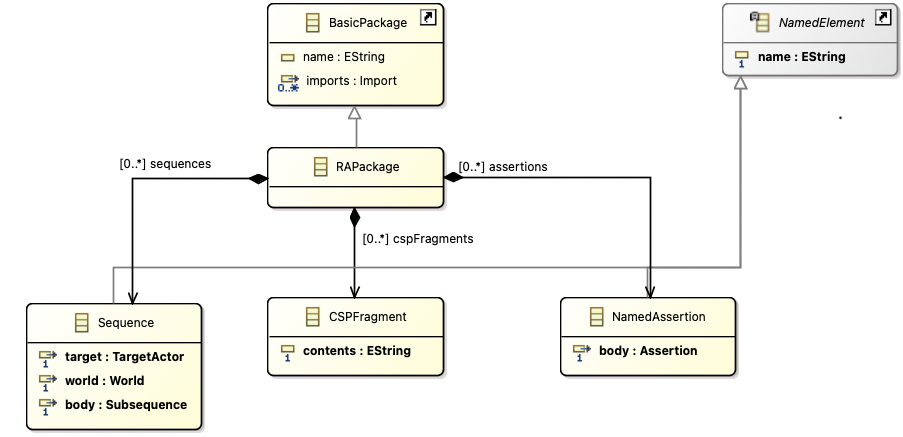
\includegraphics[width=.85\textwidth]{diagrams/top.png}
	\caption{Class diagram for the top of the \langname{} metamodel.}
	\label{fig:metamodel-top}
\end{figure}

\Cref{fig:metamodel-top} is the top-level metamodel diagram for \langname.

Each \langname{} script contains an \mrapackage,\footnote{\mrapackage{} stands
for `RoboStar Assertions package'; we use this name because \mrcpackage{} is
already used for RoboChart packages.}
which is a type of RoboStar \mbasicpackage.
Each \mrapackage{} can contain zero or more of each of these types of content:

\begin{itemize}
\item
	\msequence{}
	(\cref{sec:metamodel-sequences}):
	a sequence diagram;
\item
	\mcspfragment:
	a CSP fragment, currently not bound to a particular process
	\todo{this will change};
\item
	\massertion{}
	(\cref{sec:metamodel-assertions}):
	an assertion, currently over sequence diagrams only
	\todo{more types of assertion will appear};
\end{itemize}

\todo{Elements might need to inherit from a common class and be stored in
the same list at some point.}


\section{Sequences}\label{sec:metamodel-sequences}

\begin{figure}
	\centering
	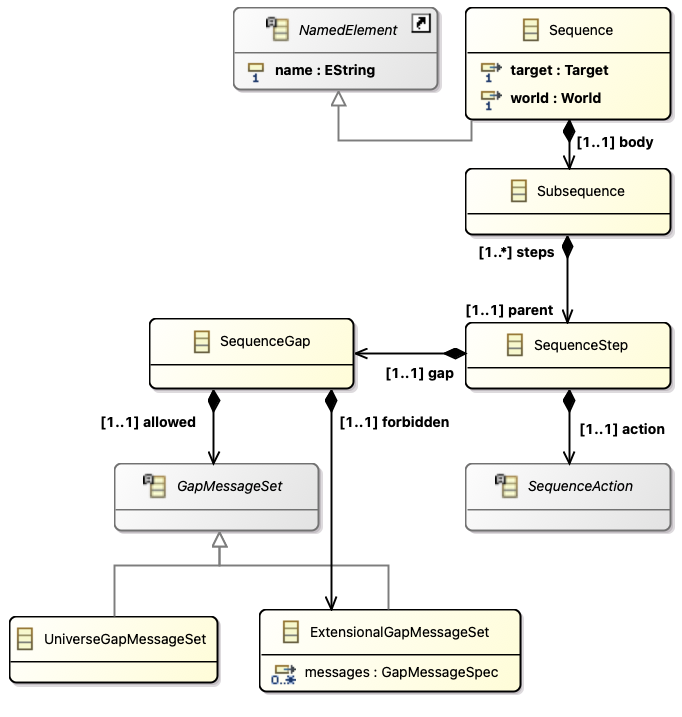
\includegraphics[width=0.7\textwidth]{diagrams/sequences.png}
	\caption{Class diagram for the part of the \langname{} metamodel dealing with sequences.}
	\label{fig:metamodel-sequences}
\end{figure}

\Cref{fig:metamodel-sequences} depicts the part of the metamodel concerning
sequence diagrams and their high-level structure.

\subsection{\msequence}

A \msequence{} represents a sequence diagram.  It is a \mnamedelement{}
that contains:

\begin{itemize}
\item
	a \msubsequence{} (\cref{ssec:metamodel-sequences-subsequences})
	containing the body of the diagram;
\item
	two \mactor s (\cref{sec:metamodel-actors}):
	a \mtarget{} (\cref{ssec:metamodel-actors-target})
	and a \mworld{} (\cref{ssec:metamodel-actors-world}).
\end{itemize}

\begin{lstlisting}[style=Example]
sequence Example
  for module ModuleName as M,  // RCModuleTarget actor
      world             as W   // World actor
{
    anything until end  // Subsequence
}
\end{lstlisting}

\subsection{\msubsequence}\label{ssec:metamodel-sequences-subsequences}

A \msubsequence{} is a sequential composition of one or more \msequencestep s
(\cref{ssec:metamodel-sequences-steps}).
All \msequence s contain exactly one \msubsequence{} at the top level, but
may contain multiple nested \msubsequence s introduced by constructs such as
\mloopaction s.

\begin{lstlisting}[style=Example]
{
    anything until operation O1() from M to W  // SequenceStep
then
    operation O2() from M to W                 // SequenceStep
then
    end                                        // SequenceStep
}
\end{lstlisting}

\subsection{\msequencestep}\label{ssec:metamodel-sequences-steps}

A \msequencestep{} is a single step in a \msubsequence.  It consists of a
\msequencegap{} (\cref{ssec:metamodel-sequences-gaps}) and a
\msequenceaction{} (\cref{sec:metamodel-actions}).

\begin{lstlisting}[style=Example]
anything until operation O() from M to W
// SequenceStep with explicit SequenceGap and SequenceAction

operation O() from M to W
// SequenceStep with explicit SequenceAction only;
// implicit SequenceGap with empty allow set
\end{lstlisting}

\subsection{\msequencegap}\label{ssec:metamodel-sequences-gaps}

A \msequencegap{} represents a condition on any communication\footnote{In PSCs,
this would correspond to \emph{intraMSG}s.} that can happen
\emph{before} a \msequenceaction.  
It contains two \mgapmessageset s: one specifying the messages
\emph{allowed} to pass inside the gap, and another specifying the messages
\emph{forbidden} to pass.\footnote{The \emph{forbidden} set is always an
\mextensionalgapmessageset, as any gap with a universal
\emph{forbidden} set would always be equivalent to one with an empty
\emph{allowed} set.
}

\begin{lstlisting}[style=Example]
anything
    in     { operation O1() from M to W   // allowed ExtensionalGapMessageSet
           , operation O2() from M to W }
    // a UniverseGapMessageSet is implied for the allow set
    // if 'in {..}' is omitted;

    except { operation O2() from M to W } // forbidden ExtensionalGapMessageSet
    // an empty ExtensionalGapMessageSet is implied for the forbidden set
    // if 'except {..}' is omitted
until // only permits O1
\end{lstlisting}

\subsection{\mgapmessageset}\label{ssec:metamodel-sequences-gap-message-sets}

A \mgapmessageset{} is an expression of the set of messages allowed or forbidden
inside a \msequencegap.  There are two types of \mgapmessageset:

\begin{itemize}
\item
	a \muniversegapmessageset{} represents the universal set containing 
	all possible messages, and
	captures a lack of specific restriction on
	the \emph{allowed} set of a \msequencegap;
\item	
	an \mextensionalgapmessageset{} is a set (expressed as an unordered list) of
	zero or more \mgapmessagespec s, themselves
	a type of \mmessagespec{} (\cref{sec:metamodel-messages}).
\end{itemize}

There is not yet any meaningful extra data stored in
\mgapmessagespec s that is not present in \mmessagespec s, but this is subject
to change.

\begin{lstlisting}[style=Example]
    universe                        // UniverseGapMessageSet
    { operation O1() from M to W }  // ExtensionalGapMessageSet
\end{lstlisting}


\section{Actions}\label{sec:metamodel-actions}

\begin{figure}
	\centering
	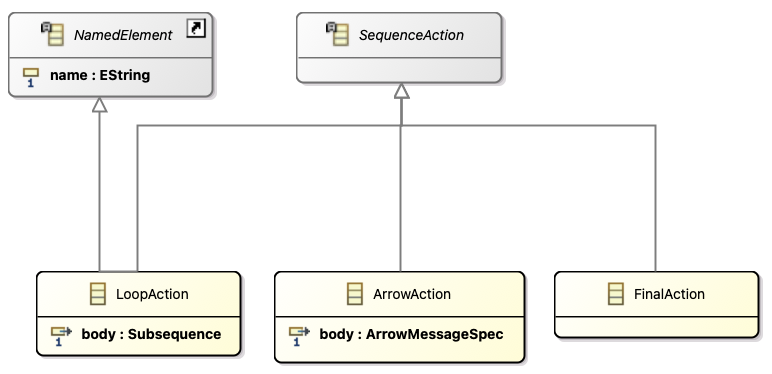
\includegraphics[width=0.7\textwidth]{diagrams/actions.png}
	\caption{Class diagram for the part of the \langname{} metamodel dealing with actions.}
	\label{fig:metamodel-actions}
\end{figure}

\Cref{fig:metamodel-actions} depicts the part of the metamodel concerning
sequence actions.

A \msequenceaction{} is an explicit communication or control flow construct in a
\msubsequence.  There are currently three types of action: arrow, loop, and
final actions.

\subsection{\marrowaction}

An \marrowaction\footnote{The name signifies both that the actions resemble
PSC \emph{arrowMSG} specifications, and also that they correspond to arrows in
the graphical syntax.} specifies one communication between \mactor s which is on
the sequence specified by the diagram.  Each \marrowaction{} wraps one
\marrowmessagespec{} (\cref{sec:metamodel-messages})
containing the specification proper.
\todo{Eventually these will bind arguments.}

\begin{lstlisting}[style=Example]
operation O1() from M to W
\end{lstlisting}

\subsection{\mloopaction}

A \mloopaction{} is a \emph{named} infinite loop.  \todo{Breaking and perhaps
other forms of loop are forthcoming.}  Each \mloopaction{} contains one
\msubsequence{} of steps to repeat indefinitely.

\begin{lstlisting}[style=Example]
loop L {
    operation O2() from M to W  // Subsequence
}  // infinite LoopAction (taking a Subsequence)
\end{lstlisting}

\subsection{\mfinalaction}

A \mfinalaction{} captures the successful termination of a sequence diagram.
A diagram with a \mfinalaction{} specifies a complete sequence of behaviour
from the \mtarget{} initialising to the \mtarget{} terminating.  Conversely,
sequence diagrams without \mfinalaction s capture partial specifications of
behaviour, or the behaviour of \mtarget s that do not terminate.

Note that the final \msequencegap{} before a \mfinalaction{} captures
any permitted communications after the behaviour explicitly specified by the
diagram has occurred.

\begin{lstlisting}[style=Example]
end
\end{lstlisting}


\section{Messages}\label{sec:metamodel-messages}

\begin{figure}
	\centering
	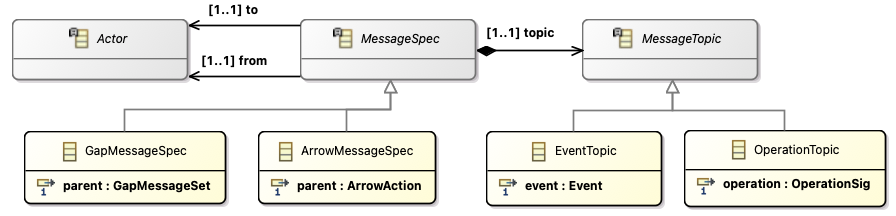
\includegraphics[width=\textwidth]{diagrams/messages.png}
	\caption{Class diagram for the part of the \langname{} metamodel dealing with messages.}
	\label{fig:metamodel-messages}
\end{figure}

\Cref{fig:metamodel-messages} depicts the part of the metamodel concerning
messages between actors.  Messages are introduced into a sequence diagram
in \mgapmessageset s and \marrowaction s.

\subsection{\mmessagespec}

A \mmessagespec{} is a specification on the types of communication that can
happen during a gap (a \mgapmessagespec) or arrow (an \marrowmessagespec).\footnote{
This class distinction resembles that in PSCs betweeen intraMSGs and arrowMSGs,
respectively.}  Each \mmessagespec{} contains:

\begin{itemize}
\item
	references to two \mactor s (\cref{sec:metamodel-actors}),
	capturing the source (\emph{from}) and destination (\emph{to})
	of the communication;
\item
	the \mmessagetopic{} (\cref{ssec:metamodel-messages-topics}) specifying
	the type of communication that the spec is capturing.
\end{itemize}

\begin{lstlisting}[style=Example]
operation O1() from M to W  // MessageSpec with OperationTopic
                            //   from actor M to actor W
event E        from W to M  // MessageSpec with EventTopic
                            //   from actor W to actor M
\end{lstlisting}

\subsection{\mmessagetopic}\label{ssec:metamodel-messages-topics}

A \mmessagetopic{} identifies the specific type of communication in a
\mmessagespec{}.  There are currently two types of topic, corresponding to
\robochart{} operations (\moperationtopic) and events (\meventtopic).
Each contains a reference to the signature of the respective construct.
Parameterised operations and events are not yet supported \todo{this will
change}.

\begin{lstlisting}[style=Example]
operation O1() // OperationTopic
event E        // EventTopic
\end{lstlisting}

\subsection{\margument}\label{ssec:metamodel-messages-arguments}

A \margument{} is a pattern that specifies (and possibly binds) one or more
arguments in
a message.  There are two types of argument:

\begin{itemize}
\item
	\mexpressionargument, which specifies that the argument is equal to the
	value of a particular \robochart{} expression;
	\todo{the CSP generator doesn't yet properly protect against this being
	an expression not expressible as a prefix}
\item
	\mrestargument, which matches \emph{all} following arguments and permits
	them to be any value.
	\todo{This mainly exists because it's very easy to specify in CSP.  Ideally
	we'll have something that allows wildcards on arbitrary parameters, in
	which case this might be confusing to have also.}
\end{itemize}

All \margument s, at time of writing, are forms of \mnonbindingargument{} and
can therefore appear in \mgapmessagespec s.  This will change when binding
arguments are introduced.

\begin{lstlisting}[style=Example]
42  // ExpressionArgument containing integer literal
... // RestArgument
\end{lstlisting}

\section{Actors}\label{sec:metamodel-actors}

\begin{figure}
	\centering
	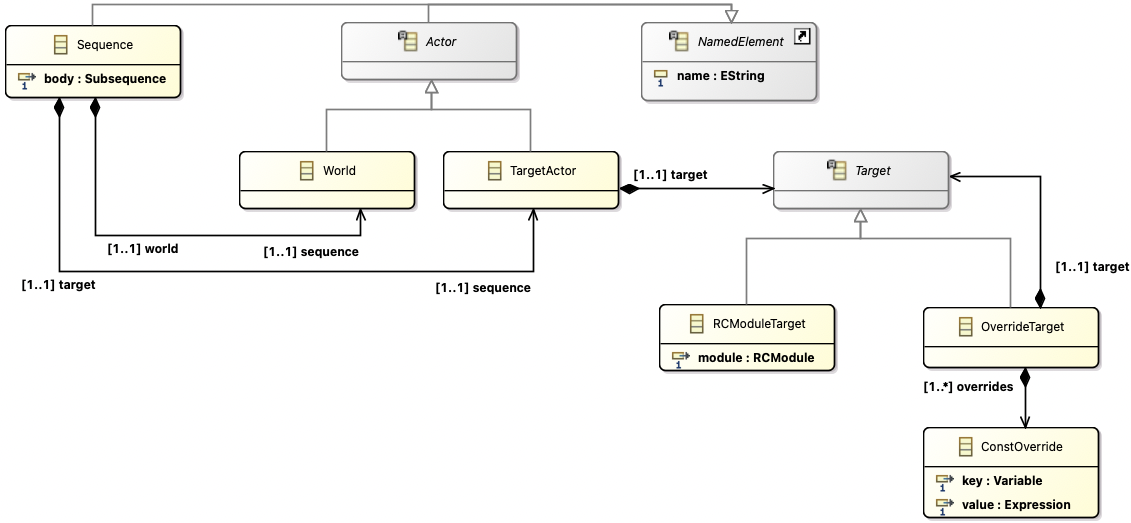
\includegraphics[width=\textwidth]{diagrams/actors.png}
	\caption{Class diagram for the part of the \langname{} metamodel dealing with actors.}
	\label{fig:metamodel-actors}
\end{figure}

\Cref{fig:metamodel-actors} depicts the part of the metamodel concerning
actors.

\subsection{\mactor}

An \mactor{} is a named participant in a sequence.  The names can be used to
specify the source and recipient of communications in \mmessagespec{}s.
As mentioned in
\cref{sec:metamodel-sequences}, there are always two actors
attached to a sequence: a \mtarget{} (\cref{ssec:metamodel-actors-target})
and a \mworld{} (\cref{ssec:metamodel-actors-world}).

\subsection{\mtarget}\label{ssec:metamodel-actors-target}

A \mtarget{} references the part of a robotic system that serves as the focus
for a particular sequence diagram.  There is
presently one type of target, with more to appear later:

\begin{itemize}
\item
	a \mrcmoduletarget{} references a \mrcmodule.
\end{itemize}

All forms of \mtarget{} contain a \mtargetinstantiation{} (see below), which
is always applied to any use of that target; assertions may further instantiate
any constants left open by the target's \mtargetinstantiation.

\begin{lstlisting}[style=Example]
module ModuleName as M
// RCModuleTarget with implicit empty TargetInstantiation

module ModuleName
    with { SOME_CONSTANT set to 4, ANOTHER_CONSTANT set to 5 }
    as M
// RCModuleTarget with explicit TargetInstantiation
\end{lstlisting}

\subsection{\mtargetinstantiation}

A \mtargetinstantiation{} instantiates some or all of the constants in the
target's parametrisation.  It contains a list of key/value pairs where each key
is a RoboChart \mvariable{} corresponding to a constant, and each value is a
RoboChart \mexpression{} evaluated in an arbitrary \todo{check this} scope.

\begin{lstlisting}[style=Example]
{ SOME_CONSTANT set to 4, ANOTHER_CONSTANT set to 5 }
\end{lstlisting}

\subsection{\mworld}\label{ssec:metamodel-actors-world}

A \mworld{} is an \mactor{} that represents the `world' outside a sequence's
\mtarget.  \mworld s do not contain any data.

\begin{lstlisting}[style=Example]
world as W
\end{lstlisting}


\section{Assertions}\label{sec:metamodel-assertions}

\begin{figure}
	\centering
	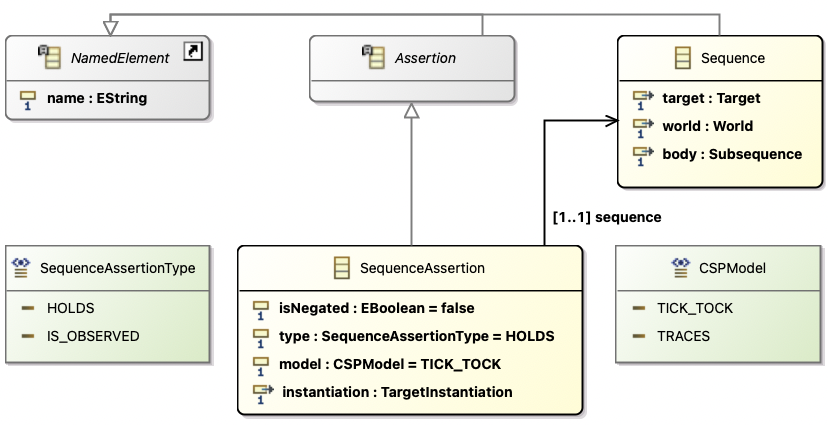
\includegraphics[width=0.7\textwidth]{diagrams/assertions.png}
	\caption{Class diagram for the part of the \langname{} metamodel dealing with assertions.}
	\label{fig:metamodel-assertions}
\end{figure}

\Cref{fig:metamodel-assertions} depicts the part of the metamodel concerning
assertions.

\subsection{\massertion}

An \massertion{} is an named assertion statement.  Currently, there is
only one type of assertion: a \msequenceassertion{}.  \todo{This will change
when merging with the existing language, if not sooner.}

\subsection{\msequenceassertion}\label{ssec:metamodel-assertions-sequence}

A \msequenceassertion{} is an assertion about a particular \msequence{} with
respect to its \mtarget.  The \mtarget{} is modified by applying an
assertion-level \mtargetinstantiation, which may fix any constants not bound
by the sequence-level instantiation.  (The default is an empty instantiation,
meaning the target is exactly as specified at the sequence level.)

The specific sequence assertion type comes from the \msequenceassertiontype:
either `sequence holds on target' (refinement), or `sequence is observed on
target' (reverse refinement).  The assertion can be negated.  The choice of
\mcspmodel{} affects how the assertion is checked with CSP tools such as FDR
\todo{the models aren't actually used yet; everything is treated as untimed
traces refinement.  This will change.}

\begin{lstlisting}[style=Example]
assertion A: SequenceName holds           // positive 'holds' SequenceAssertion
assertion B: SequenceName does not hold   // negative 'holds' SequenceAssertion
assertion C: SequenceName is observed     // positive 'is observed' SequenceAssertion
assertion D: SequenceName is not observed // negative 'is observed' SequenceAssertion

assertion E: SequenceName holds with { CONSTANT set to 5 }
// example of SequenceAssertion with custom TargetInstantiation
\end{lstlisting}
